% Requires \usepackage{graphicx}.

\begin{figure*}[tbp]
  \centering
  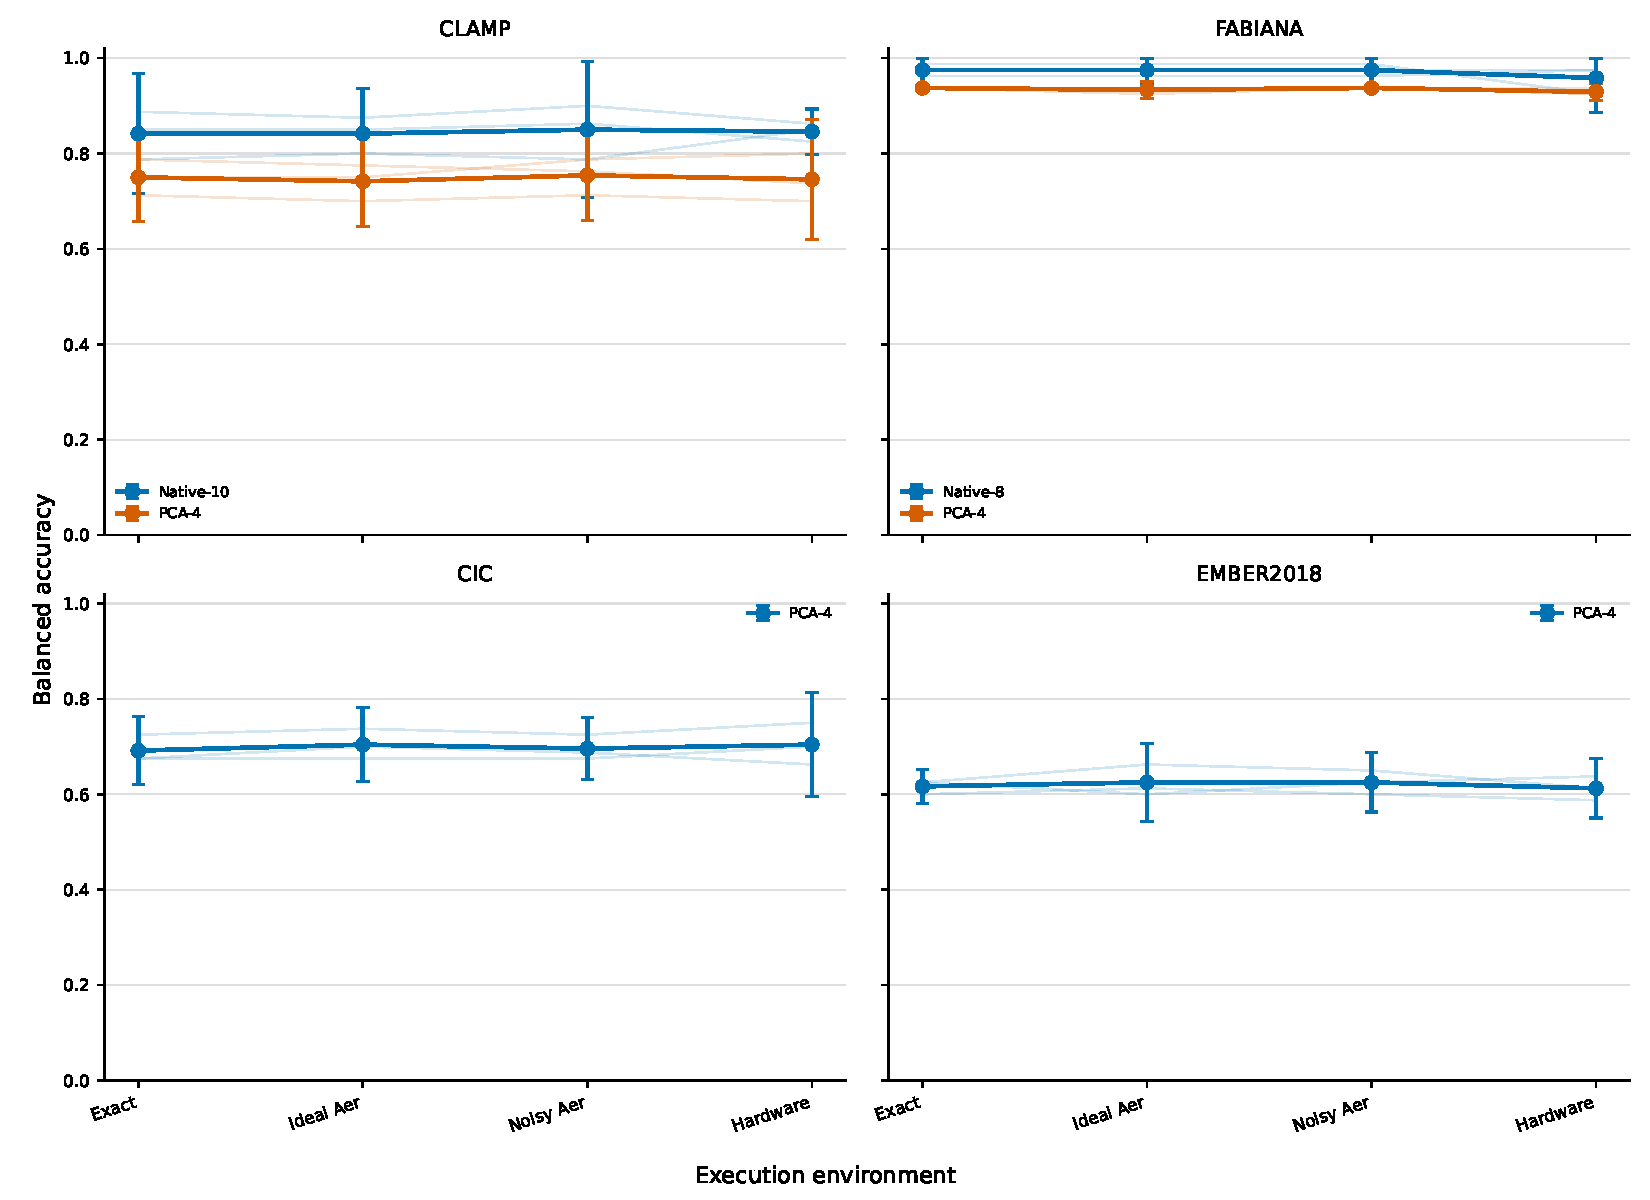
\includegraphics[width=\textwidth]{figure1_noise_ladder_balanced_accuracy.pdf}
  \caption{Balanced accuracy across exact, ideal-Aer, noisy-Aer, and IBM hardware execution. Thin lines pair held-out splits; thick lines show split means with 95\% t intervals.}
  \label{fig:noise-ladder}
\end{figure*}

\begin{figure*}[tbp]
  \centering
  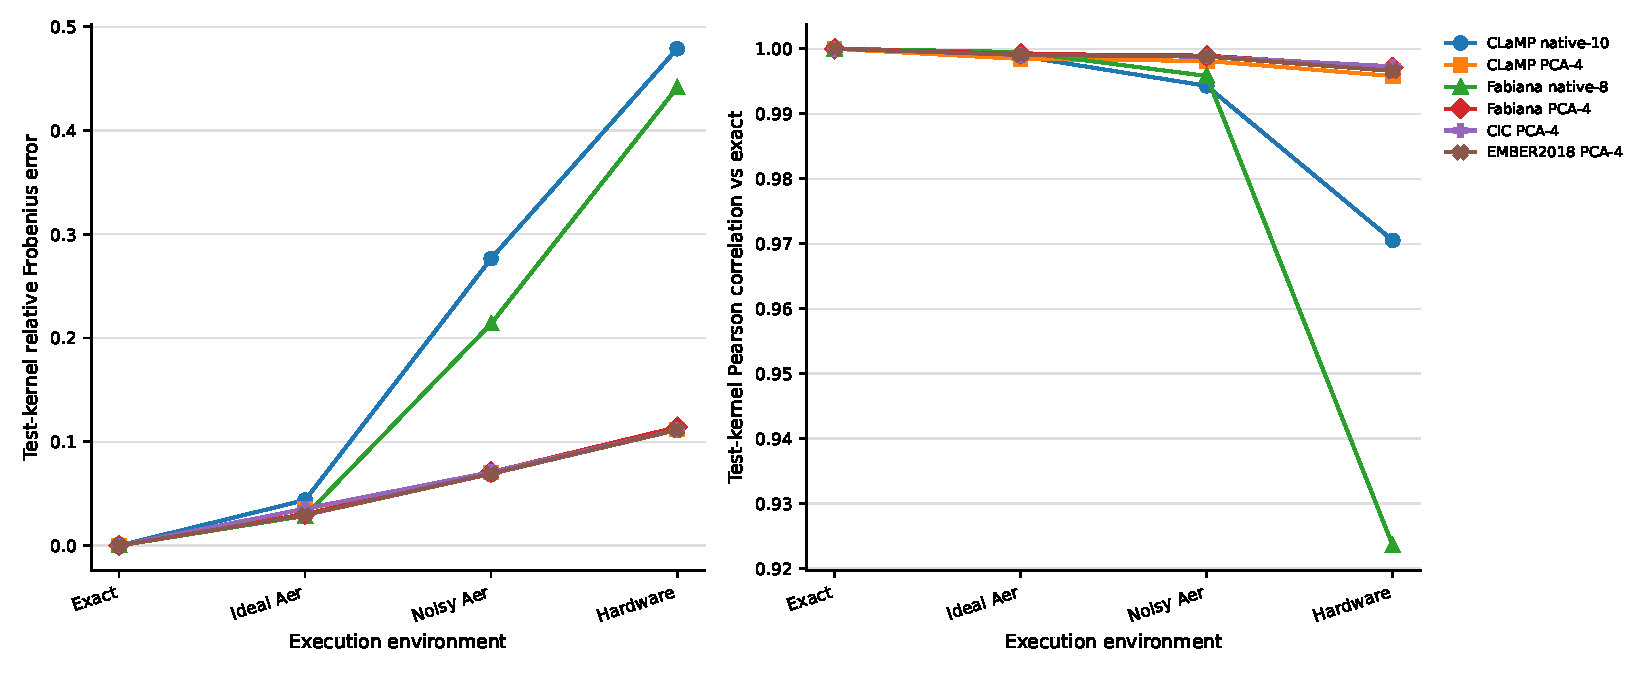
\includegraphics[width=\textwidth]{figure2_kernel_distortion.pdf}
  \caption{Test-kernel distortion relative to the exact kernel across execution environments. Lines show split-averaged relative Frobenius error and Pearson correlation.}
  \label{fig:kernel-distortion}
\end{figure*}

\begin{figure*}[tbp]
  \centering
  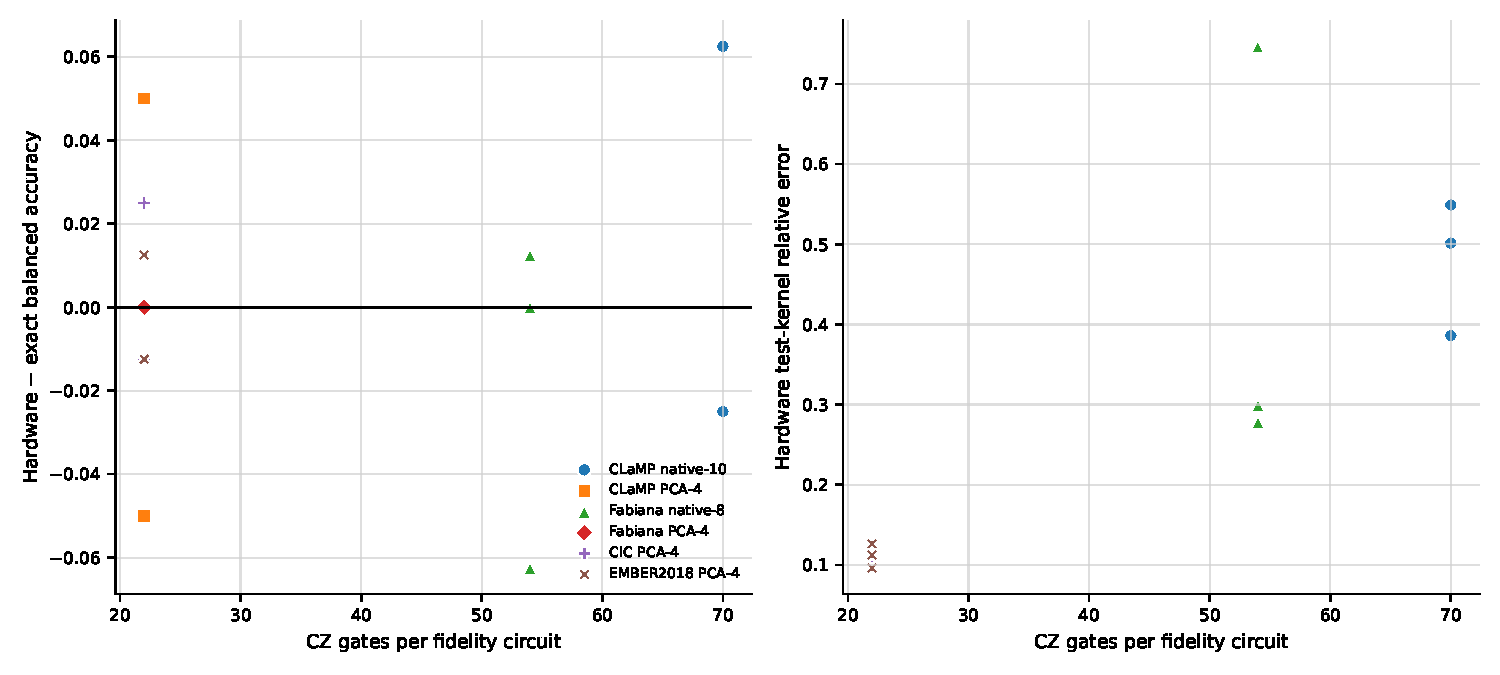
\includegraphics[width=0.92\textwidth]{figure3_circuit_cost_vs_degradation.pdf}
  \caption{Circuit cost and hardware degradation. Each point is one held-out split; CZ count is the transpiled two-qubit-gate count per fidelity circuit.}
  \label{fig:circuit-cost}
\end{figure*}
